
\begin{center}
	\textbf{\large ГЛАВА 3 \\ РЕШЕНИЕ ОБРАТНОЙ ЗАДАЧИ КИНЕМАТИКИ}
\end{center}
\refstepcounter{chapter}


% \section*{}
\addcontentsline{toc}{chapter}{ГЛАВА 3}
\section{Общее положение о механике ходьбы четырехногого робота}\label{C3_1}
Процесс движения шагающего аппарата, в котором осуществляется работа ног, можно определить как ходьбу. В ходе данного процесса каждая из ног может находиться в одном из двух основных состояний, отличающихся друг от друга принципиально.

В процессе ходьбы, ноги шагающего аппарата попеременно занимают то опорное, то свободное положения, причем в течение одного цикла каждая нога занимает то и другое положение один раз. Последовательность, в которой при ходьбе происходит чередование опорного и свободного положений всех ног аппарата, определяет конкретный способ его передвижения или его походку. Последовательность чередований ног за один период называется циклом ходьбы, а расстояние, которое проходит аппарат за один цикл, - шагом.
Движения, совершаемые любой из ног при чередовании опорного и свободного положений в процессе ходьбы, можно упрощенно разделить на фазу поступательного перемещения и фазу восстановления. В простейшем случае переход от первой фазы ко второй может осуществляться за счет движений ноги вверх-вниз строго по вертикали. Однако энергия шагающего аппарата будет расходоваться более эффективно, если в течение фазы восстановления нога будет перемещаться по некоторой кривой. Одна из возможных форм криволинейной траектории восстановления показана на рис \ref{movement}. 

Разделим предстоящую задачу формирования походки на два этапа:


\begin{figure}[h!]
	\begin{center}
		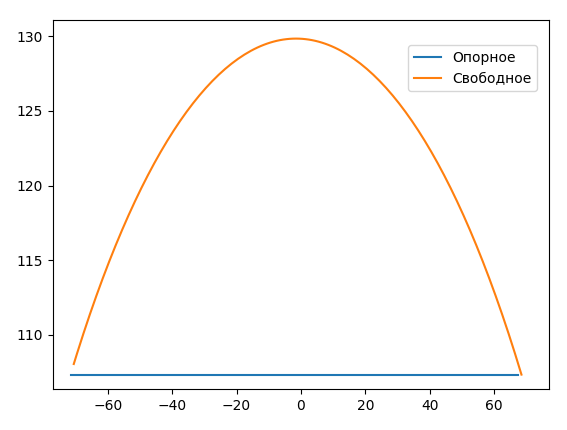
\includegraphics[width=1\textwidth]{movement}
		\caption{Фазы опорного и свободного положения ноги во время движения}
		\label{movement}
	\end{center}
\end{figure}


\begin{enumerate} 
	\item Опорное положение (перенос корпуса) - в это время нога касается поверхности и служит опорной для корпуса аппарата;
	\item Свободное положение (перенос ноги) - в это время нога находится над поверхностью и готовится к выполнению опорных функций на следующем шаге.
\end{enumerate}

\section{Решение задачи для одной ноги. Опорное положение}\label{C3_2}
Рассмотрим подробно первый этап. Нам известны длины звеньев $L_{1}$ и $L_{2}$, а также высота от поверхности земли до корпуса $h_{\text{корп}}$. 
Начальные условия для шага:
\begin{equation}
	\begin{array}{l}
		X = +X_{\text{ш}},
		\\
		Y = 0.
	\end{array}
\end{equation}
Конечные условия для шага:
\begin{equation}
	\begin{array}{l}
		X = -X_{\text{ш}},
		\\
		Y = 0.
	\end{array}
	\label{gran_step}
\end{equation}

Таким образом, положение ноги в начальный момент времени можно отобразить согласно рисунку \ref{Plus_step}
\newline
\begin{figure}[h]
	\begin{center}
		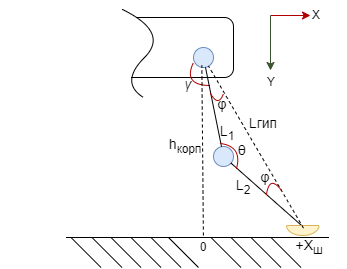
\includegraphics[width=0.6\textwidth]{Plus_step}
		\caption{Положения ноги относительно корпуса в начальный момент времени}
		\label{Plus_step}
	\end{center}
\end{figure}

В данной задаче необходимо определить закон изменения углов двигателей в бедре $\gamma$ и колене $\theta$ для положительного переноса корпуса по оси $X$. Исходя из рисунка \ref{Plus_step}, получим следующие уравнения для $\gamma$:
\begin{equation}
	\begin{array}{l}
		\phi+\gamma-\frac{\pi}{2} = \arcctg({\frac{+X_{\text{ш}}}{h_{\text{корп}}}}), 
		\\
		\gamma = \frac{\pi}{2}+ \arcctg({\frac{+X_{\text{ш}}}{h_{\text{корп}}}}) - \phi.
	\end{array}
\end{equation} 
Соответственно для $\theta$ получим:
\begin{equation}
	\begin{array}{l}
	\theta = 2 \arcsin({\frac{l_{\text{гип}}}{2l_{1}}}).
	\end{array}
\end{equation}
где вспомогательный угол $\phi$ и длину $l_{\text{гип}}$ можно найти как:
\begin{equation}
	\begin{array}{l}
		\phi=\arccos{\frac{l_{\text{гип}}}{2l_{1}}},
		\\
		l_{\text{гип}}=\sqrt{x^{2}_{\text{ш}}+h^{2}_{\text{корп}}}.
	\end{array}
\end{equation}

Далее рассмотрим конечный момент времени, где условия шага описаны формулой \ref{gran_step}. Конфигурация ноги в таком случае примет положение, которое отображено на рисунке \ref{minus_step}.
\begin{figure}[h!]
	\begin{center}
		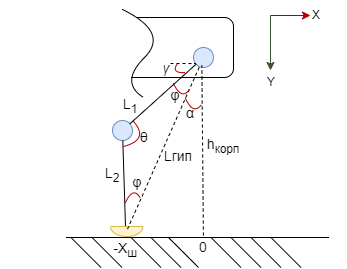
\includegraphics[width=0.6\textwidth]{minus_step}
		\caption{Положения ноги относительно корпуса в конечный момент времени}
		\label{minus_step}
	\end{center}
\end{figure}

Определим значения, которые принимают $\gamma$, $\theta$ и вспомогательный угол $\alpha$ в конечный момент времени переноса корпуса.
\begin{equation}
	\begin{array}{l}
		\gamma= \frac{\pi}{2} - \phi - \arctg({\frac{-X_{\text{ш}}}{h_{\text{корп}}}}) =
		\\
		=\frac{\pi}{2}-\arccos{\frac{l_{\text{гип}}}{2l_{1}}}+\arctg({\frac{-X_{\text{ш}}}{h_{\text{корп}}}})
		\\
		\theta = 2 \arcsin({\frac{l_{\text{гип}}}{2l_{1}}}),
		\\
		\alpha = \arctg({\frac{-X_{\text{ш}}}{h_{\text{корп}}}}),
	\end{array}
\end{equation}

Заметим, что законы изменения углов двигателей отличаются только знаком $X_{\text{ш}}$. Таким образом, определим общий закон изменения углов в зависимости от $X_{\text{ш}}$. Иначе говоря получим решение обратной задачи кинематики для одного шага робота, но без переноса стопы:
\begin{equation}
	\begin{array}{l}
		\theta(x_{\text{ш}}) = 2 \arcsin({\frac{\sqrt{x^{2}_{\text{ш}}+h^{2}_{\text{корп}}}}{2l_{1}}}),
		\\
		\gamma(x_{\text{ш}})= \frac{\pi}{2} -\arccos({\frac{\sqrt{x^{2}_{\text{ш}}+h^{2}_{\text{корп}}}}{2l_{1}}}) + \arctg({\frac{X_{\text{ш}}}{h_{\text{корп}}}}),
		\\
		l_{\text{гип}}=\sqrt{x^{2}_{\text{ш}}+h^{2}_{\text{корп}}}.
	\end{array}
	\label{finalEQ}
\end{equation}

Напишем небольшой скрипт на языке Python, чтобы построить графики изменения углов в двигателях в зависимости от ширины шага $X_{\text{ш}}$:
\newpage
\begin{python}
	
 	def callculate_step(x_range_step,height):
	
		y_step=0
		height_slew = np.sqrt(x_range_step**2+(height-y_step)**2)
		hip_step = 0.5*np.pi - np.arccos(height_slew/(2*.l1))+np.arctan(x_range_step/(height-y_step))
		knee_step = 2*np.arcsin(height_slew/(2*.l1))
	
	return np.rad2deg(hip_step), np.rad2deg(knee_step)
\end{python}

Получим следующие результаты для значений $X_{\text{ш}}$ от -40 мм до 40 мм с шагом 1 мм. Отобразим их на рисунке \ref{ideal_kin}. Для этого вызовем функцию в исполнительном файле: 


\begin{python}
	import numpy as np
	import matplotlib.pyplot as plt
	
	x_range_step = np.arange(40,-40,-10)
	hip_step = np.zeros(np.size(x_range_step))
	knee_step = np.zeros(np.size(x_range_step))

	for i in range(x_range_step):
		hip,knee = callculate_step(x_range_step[i])
		hip_step[i] = hip
		knee_step[i] = knee
	
	plt.plot(hip_step)
	plt.plot(knee_step)
	
\end{python}

\begin{figure}[h!]
	\begin{center}
		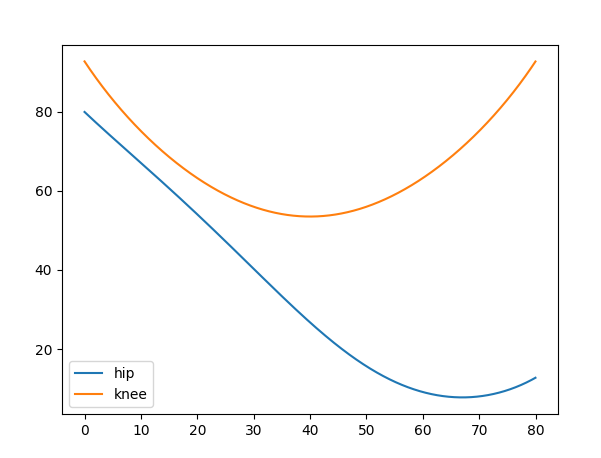
\includegraphics[width=0.9\textwidth]{ideal_kin}
		\caption{График изменения углов бедра и колена во времени}
		\label{ideal_kin}
	\end{center}
\end{figure}

\newpage 
Проверим, что в момент фазы опорного положения ноги, ее высота не изменялась и задача о положении ноги для переноса корпуса решена верно. Если задача решена верно, то результатом уравнения \ref{h_step}, при построении графика должна быть горизонтальная прямая (рисунок \ref{H} ), по значению равная $h_{\text{корп}}$, которая означает, что крайняя точка ноги (стопа) находилась на максимальном заданном расстоянии от корпуса и не изменялась в течение фазы опорного положения:
\begin{equation}
	\begin{array}{l}
		H = l_{1}\cos({\frac{\pi}{2}-\gamma}) + l_{2}\sin({\theta-\gamma})
	\end{array}
	\label{h_step}
\end{equation}
\newline
\begin{figure}[h!]
	\begin{center}
		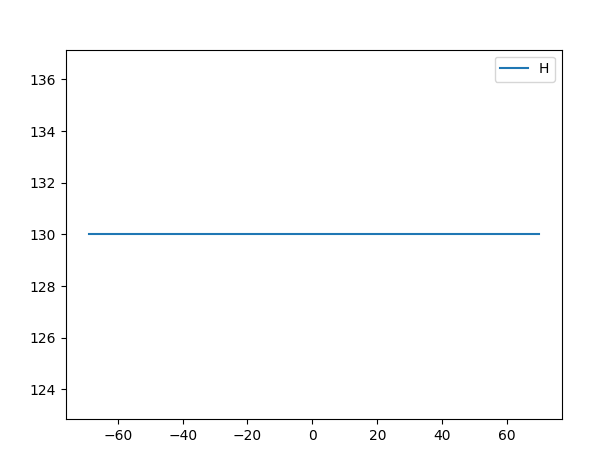
\includegraphics[width=0.9\textwidth]{H}
		\caption{График высоты стопы при опорном положении}
		\label{H}
	\end{center}
\end{figure}
\newpage
\section{Решение задачи для одной ноги. Свободное положение}\label{C3_3}
Фаза переноса - это один из ключевых этапов движения четырехногого робота, который происходит между фазами опоры. Во время переноса конечность робота находятся в воздухе и перемещается в новую позицию для следующего шага. Эта фаза требует от робота сбалансированности и точности движений, чтобы избежать падений и обеспечить плавность передвижения. Иначе говоря, фазу переноса можно рассматривать как переходный этап между двумя фазами опоры, в котором робот готовится к следующему шагу.

Рассмотрим подробно второй этап. Нам известны длины звеньев $L_{1}$, $L_{2}$ и высота от поверхности земли до корпуса $h_{\text{корп}}$. 
Условия для свободного положения включают в себя два краевых: начальное и конечное, а также серединное.
\newline
Начальные условия:
\begin{equation}
	\begin{array}{l}
		X = -X_{\text{ш}},
		\\
		Y = 0.
	\label{gran_skip1}
	\end{array}
\end{equation}
Конечные условия:
\begin{equation}
	\begin{array}{l}
		X = +X_{\text{ш}},
		\\
		Y = 0.
	\label{gran_skip2}
	\end{array}
\end{equation}
Серединные условия:
\begin{equation}
	\begin{array}{l}
		X = 0,
		\\
		Y = h_{\text{под}},
	\end{array}
	\label{gran_skip3}
\end{equation}
где $h_{\text{под}}$ - высота подъема ноги, ограничения на которую необходимо найти.
Рассмотрим кинематическую схему на рисунке \ref{skip_traj}. На нем изображена конфигурация ноги в трех положениях, которые описывают условия \ref{gran_skip1},\ref{gran_skip2},\ref{gran_skip3}. 
\newline
\begin{figure}[h!]
	\begin{center}
		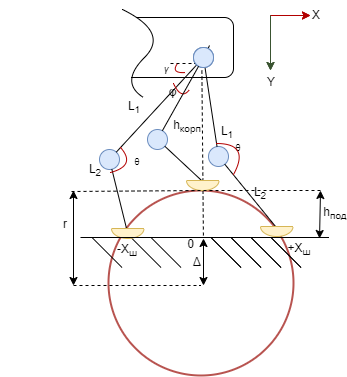
\includegraphics[width=0.6\textwidth]{skip_traj}
		\caption{Последовательность переноса стопы в свободном положении}
		\label{skip_traj}
	\end{center}
\end{figure}

С помощью регулирования радиуса $r$ создадим механизм, позволяющий регулировать высоту $h_{\text{под}}$, которая будет реализуема для заданной конфигурации робота, с учетом известных длин звеньев $l_{1}$, $l_{2}$ и высоты $h_{\text{корп}}$. Исходя из известных данных, вполне справедливо, что радиус можно найти как:
\begin{equation}
	\begin{array}{l}
		r=\sqrt{x^{2}_{\text{ш}}+\Delta^{2}} = \Delta + h_{\text{под}},
	\end{array}
	\label{radius}
\end{equation}
где $x_{\text{ш}}$ - задаваемая ширина шага от -$X_{\text{ш}}$ до $+X_{\text{ш}}$, $\Delta$ - расстояние, которым контролируется положение центра окружности по высоте.
\newline
Таким образом высота подъема стопы $h_{\text{под}}$ определяется из уравнения:
 \begin{equation}
 	\begin{array}{l}
 		h_{\text{под}}(x_{\text{ш}})=\sqrt{r^{2}-x^{2}_{\text{ш}}}-\Delta,
 		\\
 		\Delta = \sqrt{r^{2}-x^{2}_{\text{ш}}},
 	\end{array}
 	\label{hpod}
 \end{equation}
 где ограничение на высоту подъема ноги вводится как:
 \noindent $$r>x_{\text{ш}}$$
 
 Тогда с учетом найденного $h_{\text{под}}$, определим законы изменения углов в двигателях для бедра и колена соответственно:
 
 \begin{equation}
 	\begin{array}{l}
 		\theta(x_{\text{ш}}) = 2 \arcsin({\frac{\sqrt{x^{2}_{\text{ш}}+h^{2}_{\text{корп}}-h^{2}_{\text{под}}}}{2l_{1}}}),
 		\\
 		\gamma(x_{\text{ш}})= \frac{\pi}{2} -\arccos({\frac{\sqrt{x^{2}_{\text{ш}}+h^{2}_{\text{корп}}-h^{2}_{\text{под}}}}{2l_{1}}}) + \arctg({\frac{X_{\text{ш}}}{h_{\text{корп}}}}),
 		\\
 		l_{\text{гип}}=\sqrt{x^{2}_{\text{ш}}+h^{2}_{\text{корп}}},
 		\\
 		h_{\text{под}}(x_{\text{ш}})=\sqrt{r^{2}-x^{2}_{\text{ш}}}-\Delta,
 		\\
 		\Delta = \sqrt{r^{2}-x^{2}_{\text{ш}}}.
 	\end{array}
 	\label{skip_eq}
 \end{equation}
 
Аналогично с пунктом \ref{C3_2} напишем скрипт на языке Python, чтобы получить графики изменения углов в двигателях в зависимости от ширины шага $X_{\text{ш}}$:
 
 \begin{python}
	def callculate_skip(x_range_skip,min_delta,height,r):
		delta = np.sqrt(r**2-min_delta**2)
		y_skip = np.sqrt((r**2) - (x_range_skip**2)) - delta
		height_slew = np.sqrt(x_range_skip**2+(height-y_skip)**2)
		
		hip_skip = 0.5*np.pi - np.arccos(height_slew/(2*l1))+np.arctan(x_range_skip/(height-y_skip))
		knee_skip = 2*np.arcsin(height_slew/(2*l1))
		
		return np.rad2deg(hip_skip),np.rad2deg(knee_skip)
\end{python}

C учетом результатов на рисунке \ref{ideal_kin}, получим графики углов $\theta$ и $\gamma$ при переносе стопы для значений $X_{\text{ш}}$ от -40 мм до 40 мм с шагом 1 мм, высотой $h_\text{корп}$ = 130 мм и $r$ = 100 мм. Отобразим их на рисунке \ref{full_traj}. Для этого добавим функцию в исполнительный файл, описанный выше в пункте \ref{C3_2}:
\newpage
\begin{python}
	import numpy as np
	import matplotlib.pyplot as plt
	
	x_range_step = np.arange(40,-40,-10)
	x_range_skip = np.arange(-40,40,10)
	r= 100
	height = 130
	min_delta = x_range_skip[0]
	hip = []
	knee = []
	
	for i in range(x_range_step):
		hip,knee = callculate_step(x_range_step[i],height)
		hip[i] = hip
		knee[i] = knee
	
	for i in range(x_range_skip):
		hip,knee = callculate_skip(x_range_skip,min_delta,height,r)
		hip[i] = hip
		knee[i] = knee
	
	plt.plot(hip)
	plt.plot(knee)
\end{python}

\begin{figure}[h!]
	\begin{center}
		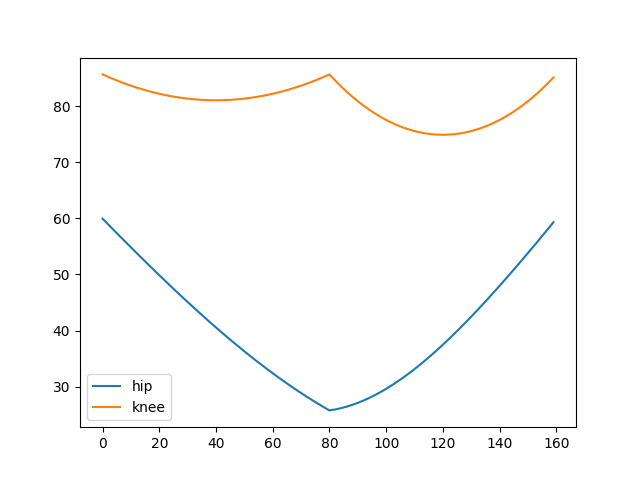
\includegraphics[width=0.8\textwidth]{full_traj}
		\caption{Изменение углов двигателей за полный цикл одного шага}
		\label{full_traj}
	\end{center}
\end{figure}
%\noindent
\newpage
Проведем проверку, аналогичную в пункте \ref{C2_2}. Если задача решена верно, то мы получим результат схожий с рисунком \ref{movement}. Для этого воспользуемся формулой \ref{h_step}. Полученный график отображен на рисунке \ref{full_cycle}

\begin{figure}[h!]
	\begin{center}
		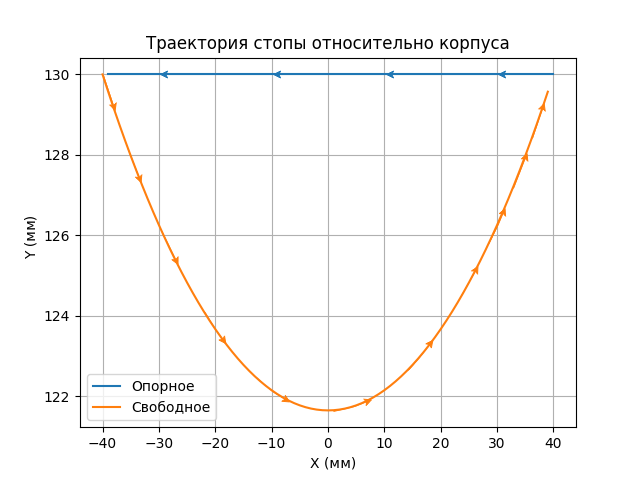
\includegraphics[width=0.9\textwidth]{full_cycle}
		\caption{Траектория стопы за полный шаг}
		\label{full_cycle}
	\end{center}
\end{figure}

\newpage